\documentclass[paper=a4, fontsize=11pt]{scrreprt}

\usepackage[T1]{fontenc}
\usepackage[german]{babel}
\usepackage{amsfonts,amsthm, amsmath}
\usepackage{siunitx}
\usepackage[]{graphicx}
\usepackage{url}
\usepackage{floatrow}
\usepackage{sectsty}
\usepackage{fancyhdr}
\usepackage[utf8]{inputenc}

\allsectionsfont{\raggedright \normalfont\scshape}
\pagestyle{fancyplain}
\fancyhead{}
\fancyfoot[L]{}
\fancyfoot[C]{}
\fancyfoot[R]{\thepage}
\renewcommand{\headrulewidth}{0pt}
\renewcommand{\footrulewidth}{0pt}
\setlength{\headheight}{13.6pt}

\numberwithin{equation}{section}
\numberwithin{figure}{section} 
\numberwithin{table}{section}

\setlength\parindent{0pt}

\newcommand{\horrule}[1]{\rule{\linewidth}{#1}}

\title{	
	\normalfont \normalsize 
	\textsc{HAW, Praktikum Rechnernetze} \\ [25pt] 
	\horrule{0.5pt} \\[0.4cm]
	\huge Protokoll 02 \\
	\horrule{2pt} \\[0.5cm]
}

\author{Sebastian Wientzek, Daniel Schruhl}

\date{\normalsize\today}
\renewcommand{\thesection}{\arabic{section}}
\sisetup{range-phrase=--}
\begin{document}

\maketitle

\section{Entwurf}

\subsection{Komponentendiagramm}

Wir haben uns für ein MVC-Pattern mit einer NetworkManager Komponente entschieden. In dieser Komponente werden die Verbindungen mit den anderen Clients und das Abarbeiten der Nachrichten des Protokolls bearbeitet.

\begin{figure}[!htb] 
  \centering
     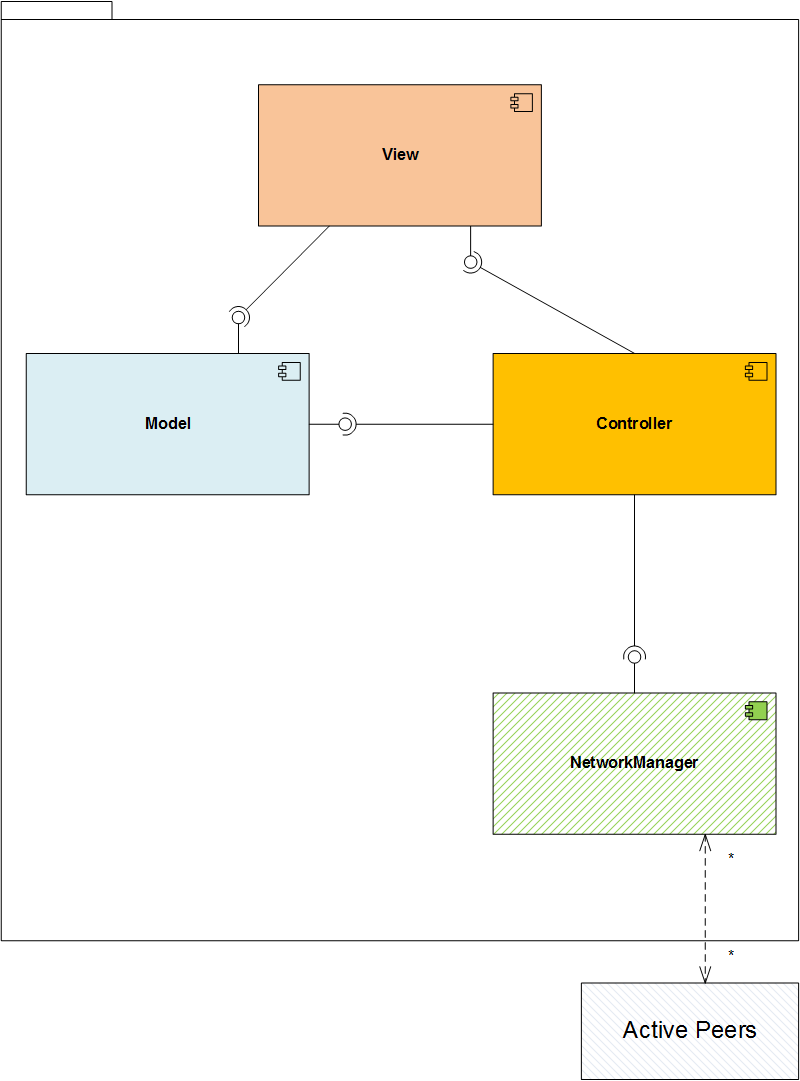
\includegraphics[width=0.7\textwidth]{resources/component-diagram.png}
  \caption{Komponentendiagramm}
  \label{fig:component-diagram}
\end{figure}

\newpage

\subsection{Aktivitätsdiagramme}

Folgende Aktivitäten sollen abgedeckt werden.

\begin{figure}[!htb] 
  \centering
     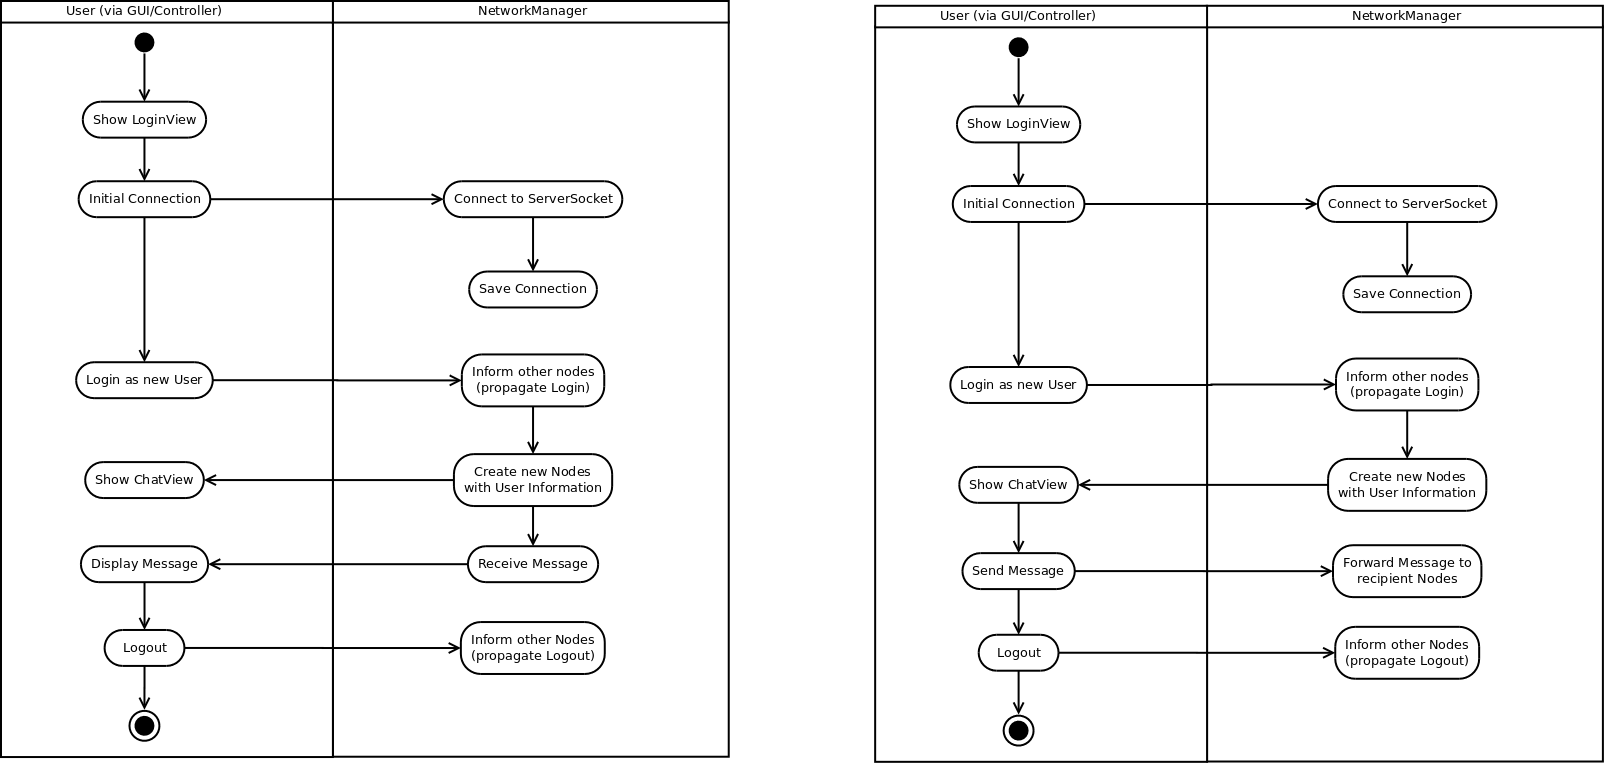
\includegraphics[width=1.0\textwidth]{resources/activity-diagram.png}
  \caption{Aktivitätsdiagramme}
  \label{fig:login-diagram}
\end{figure}

\subsection{Sequenzdiagramm}

Aus den Komponenten geben sich Sequenzdiagramme für die Fälle:

\begin{itemize}
    \item Login (Abbildung \ref{fig:login-diagram})
    \item Logout (Abbildung \ref{fig:logout-diagramm})
    \item Nachricht senden (Abbildung \ref{fig:send-diagram})
    \item Nachricht empfangen (Abbildung \ref{fig:rec-diagram})
\end{itemize}

\begin{figure}[!htb] 
  \centering
     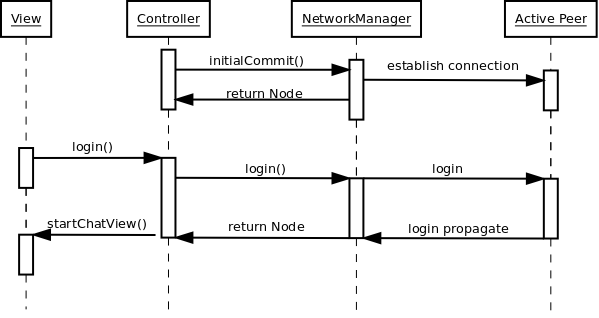
\includegraphics[width=0.7\textwidth]{resources/login-sequence.png}
  \caption{Sequenzdiagramm - Login}
  \label{fig:login-diagram}
\end{figure}

\begin{figure}[!htb] 
  \centering
     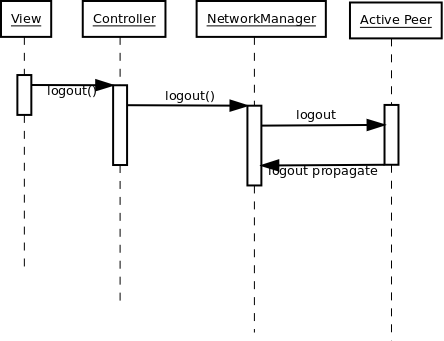
\includegraphics[width=0.7\textwidth]{resources/logout-sequence.png}
  \caption{Sequenzdiagramm - Logout}
  \label{fig:logout-diagramm}
\end{figure}

\begin{figure}[!htb] 
  \centering
     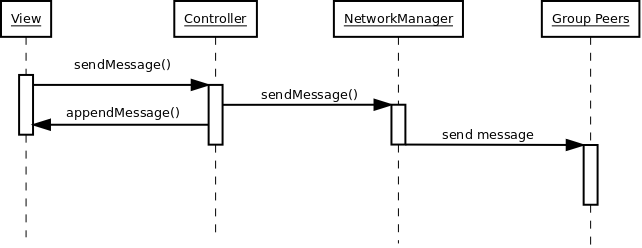
\includegraphics[width=0.7\textwidth]{resources/message-sequence.png}
  \caption{Sequenzdiagramm - Nachricht senden}
  \label{fig:send-diagram}
\end{figure}

\begin{figure}[!htb] 
  \centering
     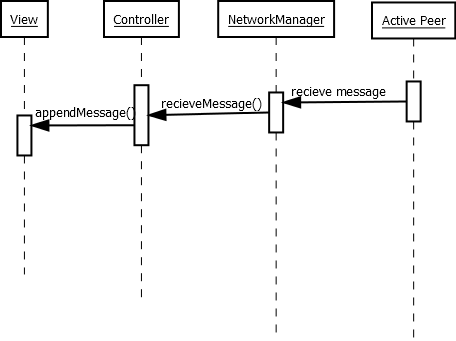
\includegraphics[width=0.7\textwidth]{resources/recieve_message-sequence.png}
  \caption{Sequenzdiagramm - Nachricht empfangen}
  \label{fig:rec-diagram}
\end{figure}

\subsection{Klassendiagramm}

Aus dem Komponentendiagramm ergibt sich das folgende Klassendiagramm (Abbildung \ref{fig:class-diagram}). Wir haben uns für das MVC-Pattern entschieden. Außerdem werden für jede Verbindung Nodes erstellt. Diese werden durch das Factory Pattern erzeugt, wodurch eine Erweiterung um das SCTP erleichtert werden soll. Außerdem wird ein Adapter verwendet, um das bearbeiten der Nachrichten zu vereinheitlichen. Dieser Handler liefert auch die User Objekte, die mit Nodes angereichert wurden. 

\begin{figure}[!htb] 
  \centering
     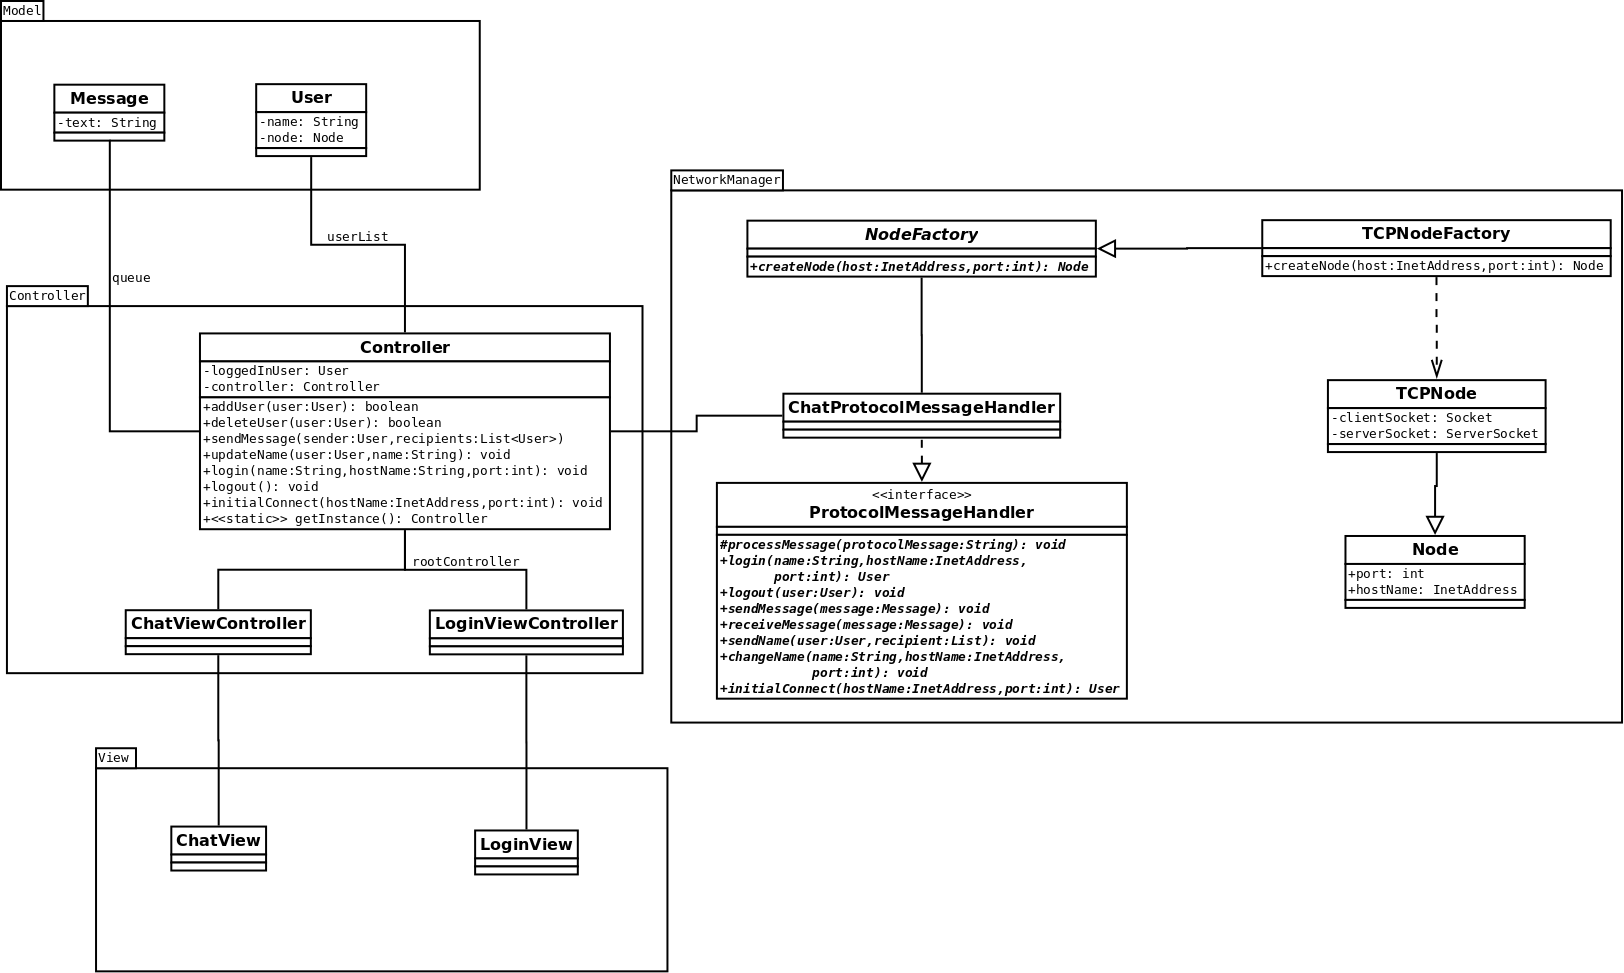
\includegraphics[width=1.0\textwidth]{resources/class-diagram.png}
  \caption{Klassendiagramm}
  \label{fig:class-diagram}
\end{figure}

\end{document}